% $Id: CONTENT.tex 12318 2010-09-24 12:03:43Z alexandra $
% Local Variables:
% ispell-check-comments: nil
% Local IspellDict: american
% End:
% --------------------------------------------------------
% User documentation
% copyright by BREDEX GmbH 2004
% --------------------------------------------------------

\app{} uses a graphical installer to make installation as straightforward as possible. 

You don't need administrative privileges to install \app{}, but the folder where the software will be installed must be writable and allow program execution.

See the following sections for information on installing \app{} on Windows and Unix systems. For installation on  other platforms, please follow the Unix installation procedure, and adapt the instructions as necessary.

\section{Environment variable: known problem}
There is a known problem with an environment variable which is installed with certain products, including other test tools, and may not be uninstalled when these products are uninstalled. 

The variable is called ''\_JAVA\_OPTION'' and causes problems for \app{} and possibly also for other Java-based software.

To see if this variable is installed on your computer, right-click on the ''my computer'' icon on your desktop and select ''properties''. 

In the dialog which appears, select the ''advanced'' tab and, at the bottom, click on the ''environment variables'' button. 

You will see a list of environment variables on the computer. 

If the ''\_JAVA\_OPTION'' variable is present, and you have uninstalled the program which used it, then you can simply remove the variable.


\section{\app{} components}


%% \begin{figure}
%% 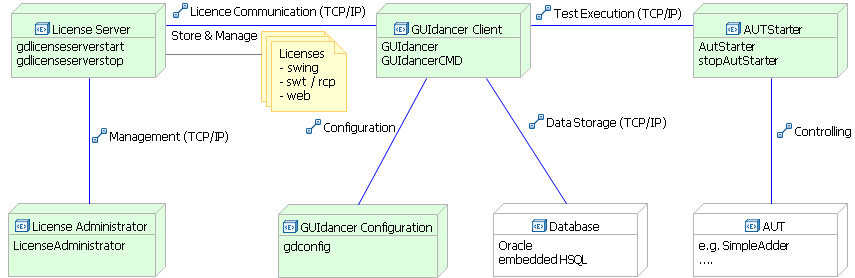
\includegraphics[width=16cm]{Installation/PS/standardInstallationDeployment}
%% \caption{\app{} components}
%% \label{gdcomponents}
%% \end{figure}

\begin{description}
\item [The Integrated Test Environment (\ite{}): ]{This is where test are created. Tests can also be executed from the client. You can think of this as the main application. The \ite{} can also run headless -- the test executor.}
\item [The \gdagent{}:]{ This component is responsible for controlling the \gdaut{} during test execution. It must be installed on the machine(s) where you want your \gdaut{} and tests to run. It requires a network connection to communicate with the \ite{}. }
\end{description}

During the installation process you can choose between different bundles of these programs to be installed:

\begin{itemize}
\item \app{}, this bundle includes
	\begin{itemize}
	\item the \ite{} and test executor
	\end{itemize}
\item \gdagent{}, this bundle includes only the \gdagent{}, which handles the testing
of your \gdaut{}.
\item \app{} Documentation, this bundle includes the PDF Documentation.
\end{itemize}


 
